\section*{سوال ۶}

سوال عملی تمرین ۱، کد شبیه‌سازی...
\section*{جواب سوال ۶}

کد ارائه شده برای شبیه‌سازی عملیات دو سرور در یک سیستم کوئیو (صف) است. سیستم دارای دو سرور با نام‌های "Able" و "Baker" است که برای پذیرش و سرویس‌دهی به مشتریان مورد استفاده قرار می‌گیرند. این شبیه‌سازی شامل موارد زیر است:

\begin{itemize}
	\item توزیع زمان بین ورودی‌ها و زمان سرویس: این داده‌ها از دو جدول توزیع احتمالاتی استخراج شده و در قالب دیکشنری‌هایی در کد قرار داده شده‌اند. زمان بین ورودی‌ها و زمان سرویس برای هر سرور مطابق با این توزیع‌های احتمالاتی تولید می‌شوند.
	\item تولید زمان بین ورودی‌ها: تابع \texttt{generate\_interarrival\_time} به صورت تصادفی زمان‌های بین ورود مشتریان را مطابق با توزیع احتمالاتی مربوطه تولید می‌کند.
	\item تولید زمان سرویس: تابع \texttt{generate\_service\_time} به صورت تصادفی زمان سرویس برای هر سرور را مطابق با توزیع احتمالاتی خودش تولید می‌کند.
	\item شبیه‌سازی: کد از طریق حلقه‌ای برای هر مشتری، بررسی می‌کند که آیا هر سرور در زمان ورود مشتری آزاد است یا خیر. اگر آزاد باشد، مشتری را سرویس می‌دهد و اگر نباشد، مشتری باید منتظر بماند.
	\item محاسبه زمان بیکاری و استفاده: برای هر سرور، کد زمان بیکاری و زمان استفاده را به صورت دوره‌ای محاسبه می‌کند. این امر از طریق ثبت زمان‌هایی که سرور بیکار است و زمان‌هایی که سرور مشغول سرویس‌دهی است، انجام می‌شود.
	\item ترسیم نمودار: کد برای هر سرور نمودارهایی از استفاده و زمان بیکاری را ترسیم و ذخیره می‌کند.
	\item میانگین استفاده و زمان بیکاری: برای هر سرور، میانگین زمان استفاده و زمان بیکاری را محاسبه و چاپ می‌کند.
\end{itemize}

\textbf{تحلیل خروجی‌ها:}

\textbf{Able :}
\begin{itemize}
	\item \textbf{\lr{Average Utilization} (میانگین استفاده):} \(0.68\) یا \(68\%\) از زمان، سرور Able مشغول سرویس‌دهی به مشتریان است. این به این معنی است که سرور اکثر اوقات فعال است و نسبتاً بار کاری بالایی دارد.
	\item \textbf{\lr{Average Idle Time} (میانگین زمان بیکاری):} \(0.32\) یا \(32\%\) از زمان، سرور Able بیکار است. این نشان‌دهنده تعادل خوبی بین زمان بیکاری و استفاده است که از کارآیی مناسب سرور حکایت دارد.
\end{itemize}

\textbf{Baker :}
\begin{itemize}
	\item \textbf{\lr{Average Utilization} :} \(0.81\) یا \(81\%\) از زمان، سرور Baker در حال سرویس‌دهی است. این بدان معنی است که سرور Baker نسبت به سرور Able فعال‌تر است و بار کاری سنگین‌تری دارد.
	\item \textbf{\lr{Average Idle Time} :} \(0.19\) یا \(19\%\) از زمان، سرور Baker بیکار است. این سرور کمترین زمان بیکاری را دارد و ممکن است نشان‌دهنده نیاز به منابع بیشتر برای جلوگیری از بیش‌باری باشد.
\end{itemize}

با توجه به این خروجی‌ها، می‌توان نتیجه گرفت که سرور Baker نیاز به توجه بیشتری دارد تا از اضافه‌بار جلوگیری شود. ممکن است لازم باشد برنامه‌ریزی برای این سرور مجدداً انجام شود تا بتواند با بار کاری کنونی خود به خوبی کنار آید یا شاید نیاز به افزایش ظرفیت یا تعداد سرورها باشد.

\begin{figure}[H]
	\centering
	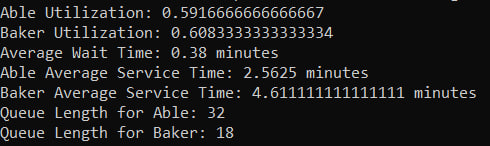
\includegraphics{pic1.jpg}
	\label{fig:label4}
\end{figure}

\begin{figure}[H]
	\centering
	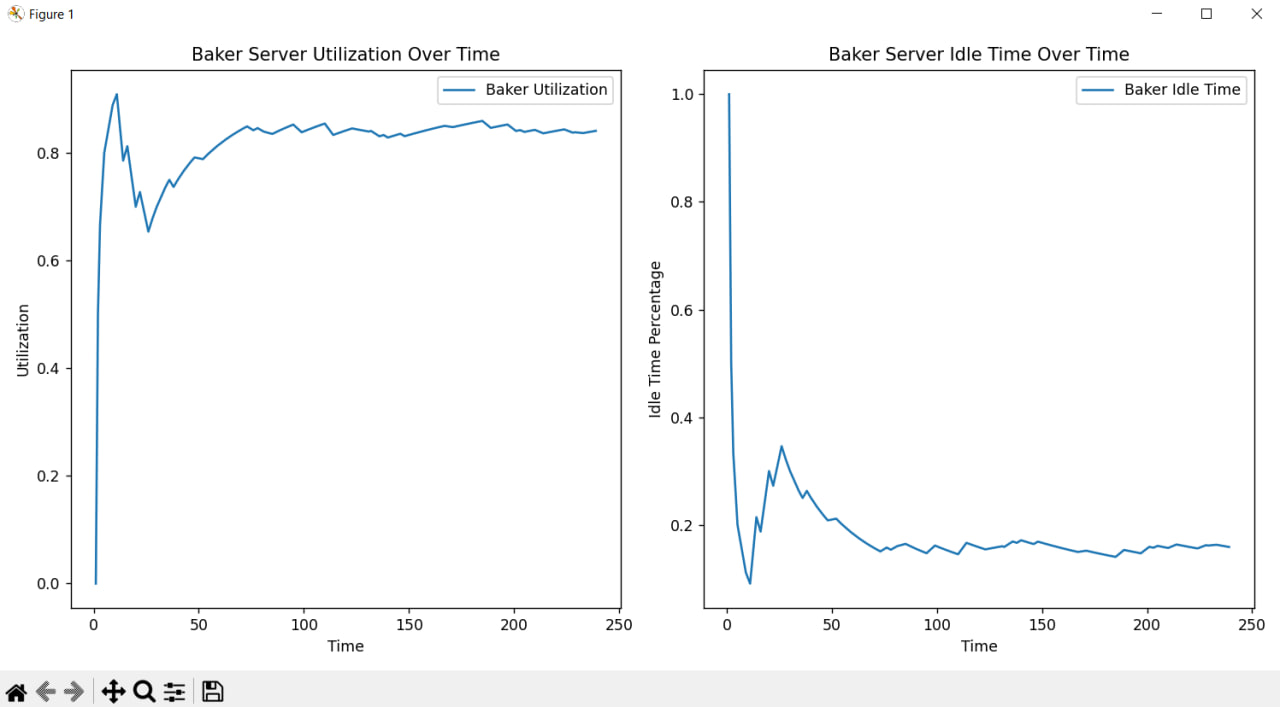
\includegraphics{pic2.jpg}
	\label{fig:label4}
\end{figure}